\documentclass[10pt, a4paper]{scrartcl}

\usepackage{vorschule}
\usepackage[
	typ=ab,
	fach=Informatik,
	lerngruppe={Q2-GK},
	nummer=II.3,
	module={Symbole,Lizenzen},
	seitenzahlen=keine,
	farbig,
	lizenz=cc-by-nc-sa-4,
]{schule}

\usepackage[
	kuerzel=Ngb,
	reihe={Rechnernetze},
	version={2020-11-03},
]{ngbschule}

\author{J. Neugebauer}
\title{Übersicht von Netzwerktopologien}
\date{\Heute}

\setzeAufgabentemplate{ngbnormal}

\begin{document}
\ReiheTitel

Die Struktur von Rechnernetzen wird in der Regel durch einen Graphen dargestellt. Die Knoten sind am Netzwerk beteiligte Geräte, die Kanten Verbindungen zwischen ihnen (zum Beispiel Netzwerkkabel, Wi-Fi, Bluetooth, ...). Diese Struktur nenn man eine \emph{Topologie}.

\begin{tabularx}{\textwidth}{|c|l|X|X|} \hline
	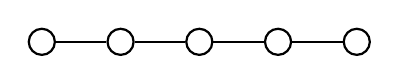
\begin{tikzpicture}
		\node[circle,black,draw,thick] (a) {};
		\node[circle,black,draw,thick,right of=a] (b) {};
		\node[circle,black,draw,thick,right of=b] (c) {};
		\node[circle,black,draw,thick,right of=c] (d) {};
		\node[circle,black,draw,thick,right of=d] (e) {};
		\draw[black,thick] (a)--(b)--(c)--(d)--(e);
	\end{tikzpicture} & lineare Topologie &&\\\hline
\end{tabularx}

\end{document}